\section{Aufgaben}
Die Aufgaben sollen die Aufnahme- und Leistungsfähigkeit der Studienteilnehmer überprüfen. Hierzu wurden Aufgaben gewählt für dessen Erledigung keinerlei Erfahrung mit Virtual-Reality Geräten vorausgesetzt wird. Die Übungen sind verständlich und auch ohne Spielerfahrung bewältigbar.
Insgesamt werden dem Probanden drei Aufgaben gestellt. 
%Jede einzelne von ihnen lässt sich durch wiederholtes, einfaches Zielen mit dem Controller und %anschließendem Betätigen einer Taste bewältigen.

% Um die Spiele zu entwickeln können aber auch Toolboxes und Frameworks herangezogen werden, so zum Beispiel auch~\cite{devisch2018mini}.
% Die validierung der Spiele gestaltet sich als schwierig, oder findet jemand noch Quellen? Kann man auch sagen, da es sich nicht um spiele handelt, gestaltet man Aufgaben, die (abstrakt) nahe an eine reale Tätigkeit herankommen? Oder kann man argumentieren, dass hier die gewählten Aufgaben einer realen Tätigkeit entsprechen?

\subsubsection{Zahlenfolge} 
Verteilt über das Blickfeld des Probanden werden Zahlen angezeigt. Die Abstände zwischen den Zahlen sind nicht gleichverteilt und werden idealerweise so gewählt, dass eine Verwechslungsgefahr besteht. Aufsteigend sollen die Zahlen selektiert und so geordnet werden. Diese Aufgabe soll das schnelle Wahrnehmen bekannter Elemente (in diesem Fall das Wahrnehmen von Zahlen) und die Fähigkeit des numerischen Sortierens Prüfen. 
%Evtl noch ein bisschen ausschmücken.
(1423 $\rightarrow$ 3177 $\rightarrow$ 4109 $\rightarrow$ 6188 ...)

\begin{figure}[H]
	\centering
	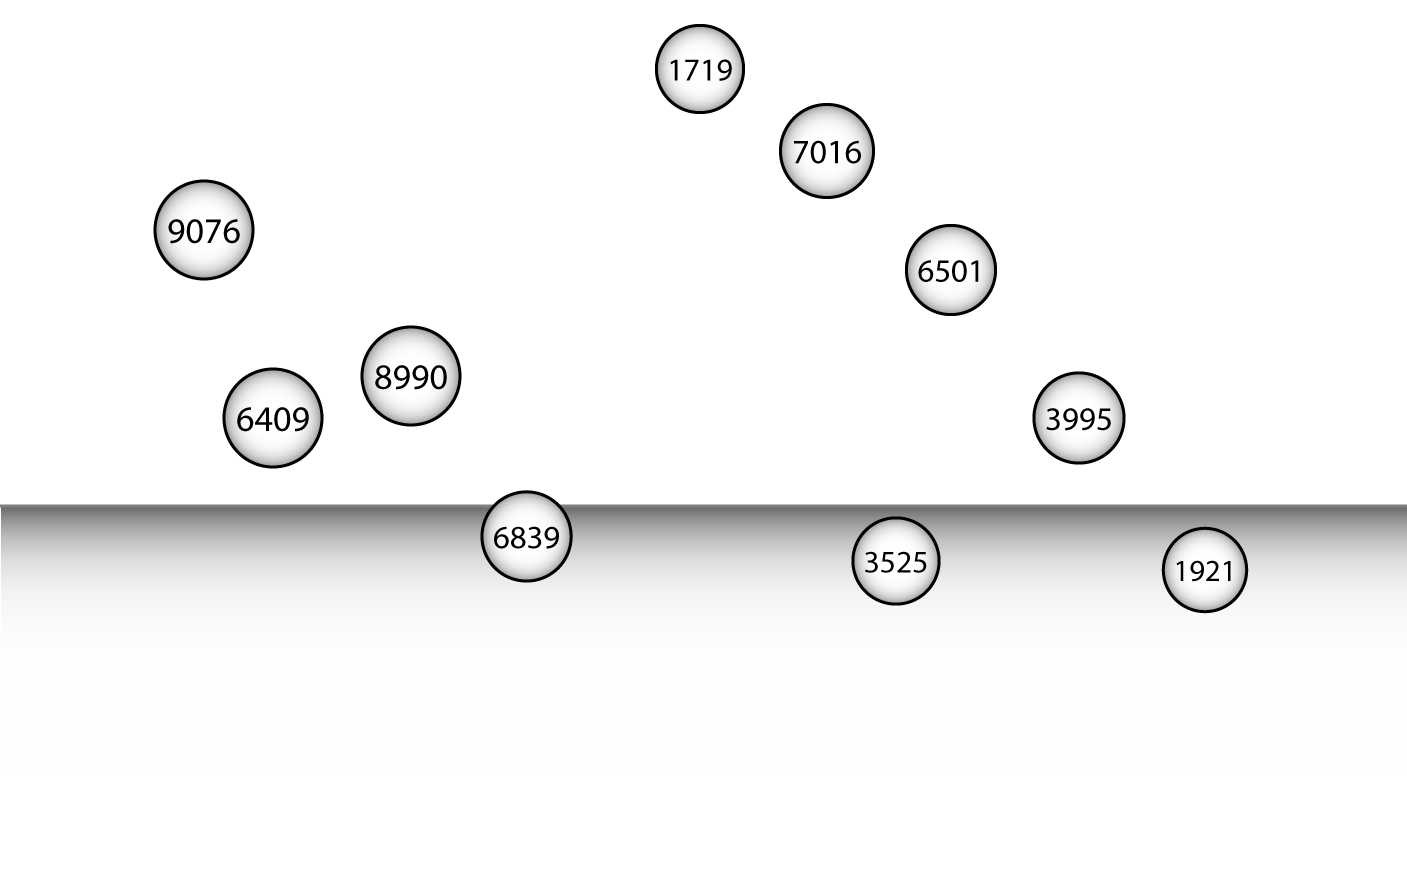
\includegraphics[width=0.8\textwidth]{./images/ordering_abstract.png}
	\caption{Erste Aufgabe der Studie. Der Text auf den Kugeln soll in aufsteigender Reihenfolge sortiert ausgewählt werden.}
	\label{fig:ordeing_abstract}
\end{figure}

\subsubsection{Stroop-Effekt} 
Im Mittelpunkt des Blickfeldes wird eine ausgeschriebene Farbe angezeigt. Die Textfarbe des Worts muss nicht zwangsläufig die der ausgeschriebenen Farbe sein. Der Proband soll als Eingabe die Textfarbe auswählen indem er mit dem Controller auf einem Interface die richtige Auswahl trifft. Beispiel kann in Figure~\ref{fig:matching_abstract} gesehen werden. Diese Aufgabe dient dem Testen von ungewohnten Aufgaben, welche dem Anwender in der Regel nicht vertraut sind und auf welche sich der Proband in kürzester Zeit einstellen muss.

\begin{figure}[H]
	\centering
	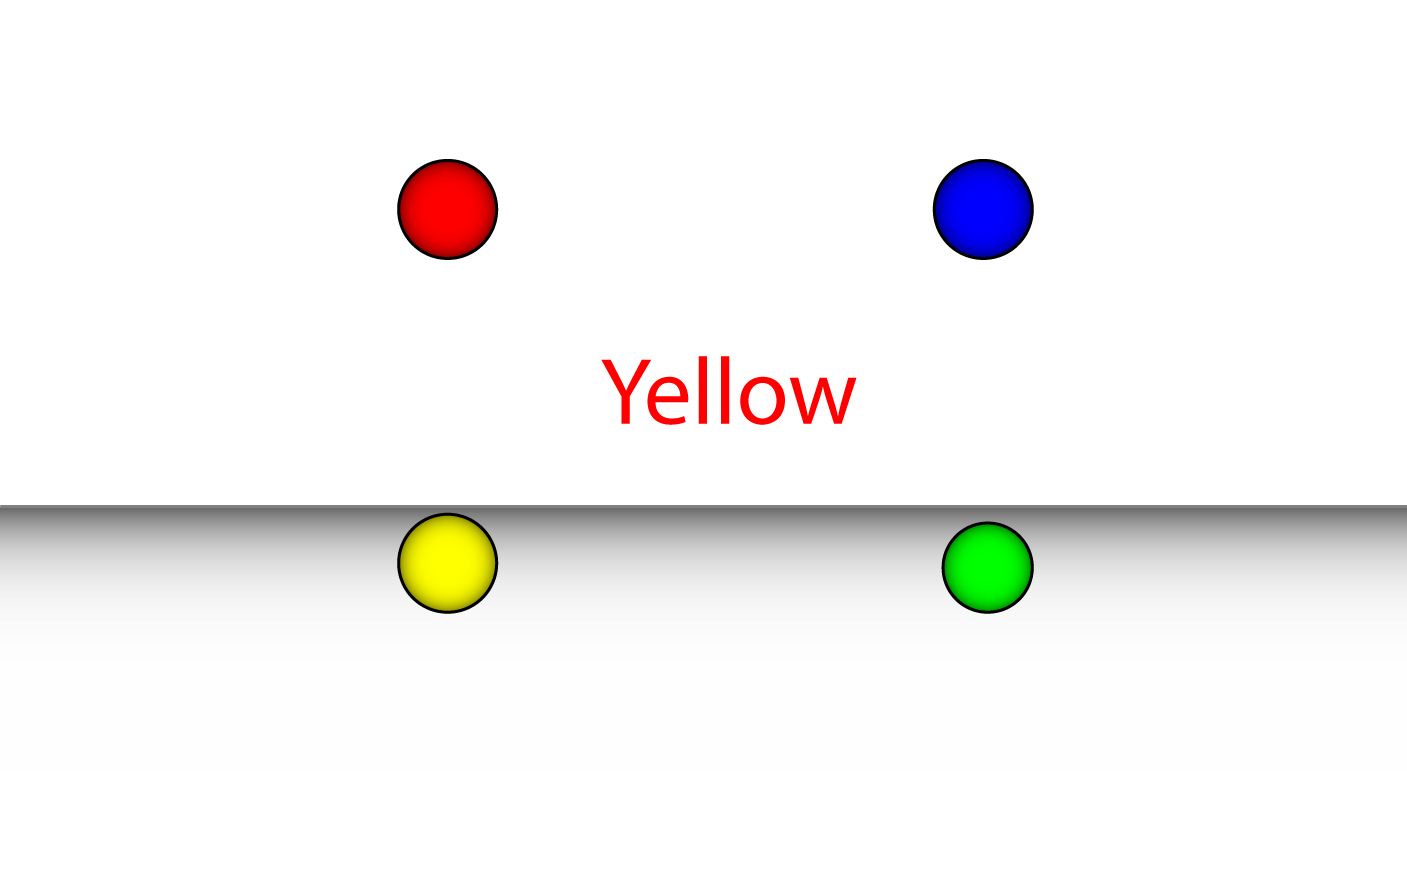
\includegraphics[width=0.8\textwidth]{./images/matching_abstract.png}
	\caption{Zweite Aufgabe. Teilnehmer der Studie sollen die Farbe, welche in Textform im Sichtbaren Bereich steht auswählen. Es soll nicht die gleiche Farbe ausgewählt werden.}
	\label{fig:matching_abstract}
\end{figure}

\subsubsection{Boxen zählen} 
In isometrischer Ansicht werden eine Vielzahl von Boxen innerhalb der virtuellen Umgebung angezeigt. Die Boxen stehen aufeinander und verdecken zum Teil den Blick auf andere Boxen. Es soll durch die Schlussfolgerung, dass diese, so wie in der realen Welt, nicht in der Luft schweben können, die Anzahl der Boxen gezählt und ausgewählt werden. Diese Aufgabe konzentriert sich auf das räumliche Wahrnehmen und Vorstellungsvermögen des Anwenders.

\begin{figure}[H]
	\centering
	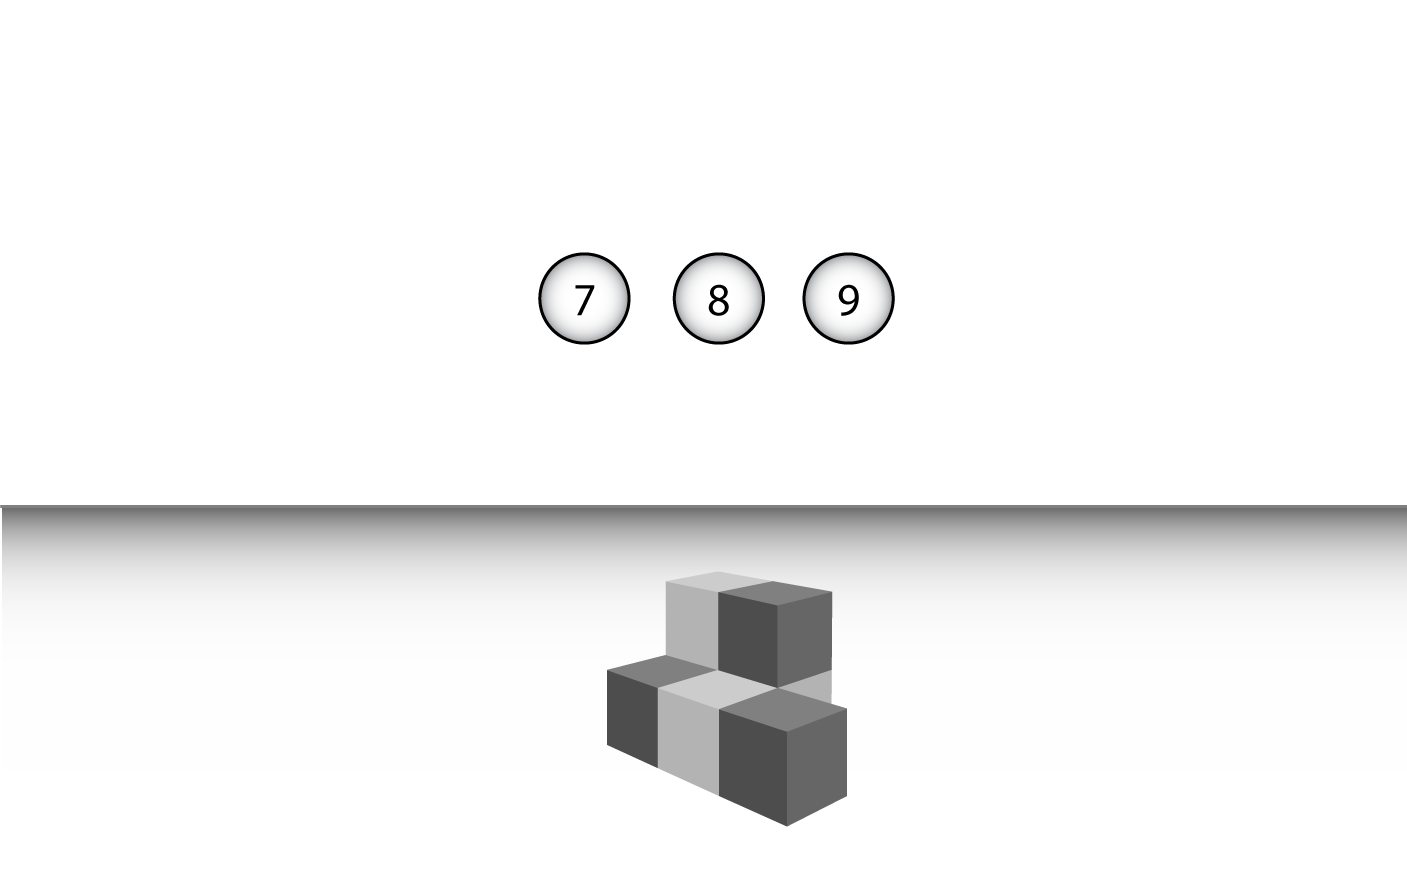
\includegraphics[width=0.8\textwidth]{./images/counting_abstract.png}
	\caption{Dritte Aufgabe in der virtuellen Umgebung. Die Teilnehmer sollen die Anzahl der Boxen zählen. Boxen verdecken die Sicht auf andere Boxen. Sie können nicht in der Luft schweben.}
	\label{fig:counting_abstract}
\end{figure}

%  ===== THIS IS INTENTIONALLY LEFT HERE AS REFERENCE FOR SUBFIGURES (copy&paste)
% \begin{figure}
% 	% \centering
% 	\begin{subfigure}{0.4\textwidth}
% 		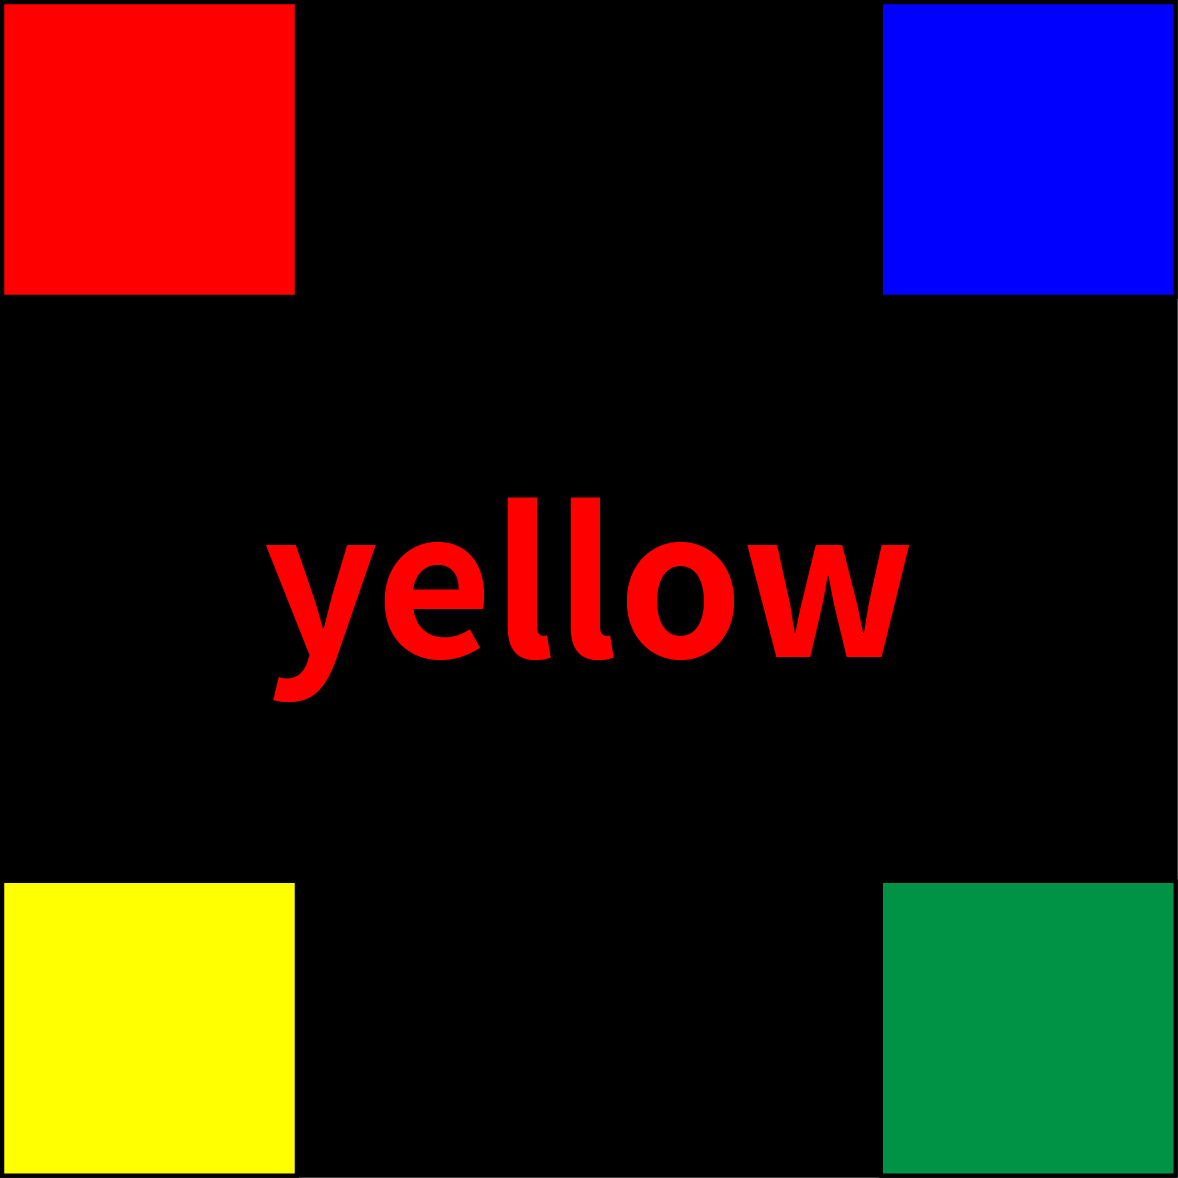
\includegraphics[width=\textwidth]{./images/Reversed_stroop_test.jpg}
% 		\caption{Stroop Test, ElvisLin CC BY-SA 4.0. \url{https://commons.wikimedia.org/wiki/File:Reversed_stroop_test.jpg}} % subcaption
% 		\label{fig:stroop_test}
% 	\end{subfigure}%
% 	\hfill
% 	\begin{subfigure}{0.5\textwidth}
% 		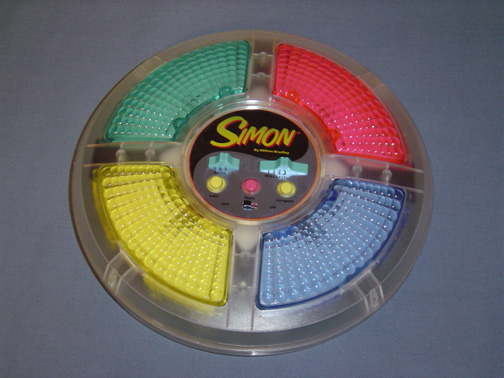
\includegraphics[width=\textwidth]{./images/Simon_game.jpg}
% 		\caption{Senso / Simon, Larry D. Moore CC BY-SA 3.0. \url{https://commons.wikimedia.org/wiki/File:Simon_game.jpg}} % subcaption
% 		\label{fig:simon}
% 	\end{subfigure}
% 	\caption{Beispiele für die Spiele mit denen die Teilnehmer konfrontiert werden.} % caption for whole figure
% \end{figure}
